\documentclass[12pt,letterpaper, singlecolumn]{article}
\usepackage{latex8}
\usepackage{times}
\usepackage{cite}
\usepackage{subfigure}
\usepackage{psfig}
\usepackage[pdftex]{graphicx}
\usepackage{epsfig}
\usepackage{pstricks}
\usepackage{fullpage}
\usepackage{amsthm}
\usepackage{graphics}
\usepackage{comment}
\usepackage[small,compact]{titlesec}
\usepackage[small,it]{caption}
\usepackage{wrapfig}

\begin{document}

\title{CSE530 Project Mid-Point Progress Report\\
Bandwidth-Aware Memory Hierarchy Design with Hybrid Memory Technologies}

\author{Cong Xu and Jishen Zhao\\
\{czx102, juz138\}@psu.edu\vspace{-10pt}
}
\maketitle

\begin{large}

% ------------------------------------------------------------------------------

\section{Project Description}

One of the challenges for modern chip-multiprocessor~(CMP) design is the growing bandwidth gap
between processor cores and off-chip main memory. Emerging memory technologies
bring in potential opportunities to fill this gap. The memory hierarchy,
however, need to be carefully designed in order to bridge the this gap with low
performance and power overhead.

In this project, we would like to explore the optimal memory hierarchy design
with various memory technologies specifically for bandwidth-bounded
applications. We will first estimate the performance of an application on a
baseline system, in terms of the bandwidth demanded by the application for a
range of memory capacities and the bandwidth that can be provided by the system
with such memory capacities. We would like to find out whether the bandwidth
provided by the memory hierarchy can satisfy the demand. If it is not satisfied,
we can modify the memory hierarchy, for example, by changing the capacity of
existing cache and memories, or by adding an extra level of cache or memory.
Based on our exploration, we would like to find a memory hierarchy design
solution optimized for bandwidth, including the number of cache and memory
levels, as well as the memory technology, the bandwidth, and the capacity used
for each level. In addition, we will enhance the memory hierarchy design from
the energy-efficiency point of view by constraining the total power consumption
of the memory system.\vspace{0.15in}

% ------------------------------------------------------------------------------

\section{Motivation}

Many of modern chip-multiprocessors are designed to perform well on various
applications to achieve high performance by exploiting their inherent
parallelism. Such systems support large number of threads and single instruction
multiple data~(SIMD) execution, which puts a lot of pressure on the memory
system. Memory latency is typically not a bottleneck, since the latency can be
hidden via multi-threading or hardware prefetching. To this end, bandwidth becomes a
potential bottleneck. A high rate of computing often brings in a high rate of
data transitions. In some cases, the working set of an application fits in the
on-die caches, which can typically provide sufficient bandwidth to keep up with
the processing cores. However, if the working set does not fit in the on-die
caches, the main memory needs to provide much of the data. Since the bandwidth
of off-chip main memory is quite limited, applications with such working sets
are potentially bandwidth-bound. Therefore, it is crucial to design the memory
hierarchy to overcome the bandwidth limitation. 

It is known that performance improvement of a computing system can be achieved
via multiple memory levels. Adding an extra level of memory, however, can also
help alleviate the bandwidth bottleneck of off-chip memory. In addition,
emerging memory technologies such as Magnetoresistive Random Access
Memory~(MRAM), Phase-Change Memory~(PCM), Resistive Random Access Memory~(RRAM),
etc., have shown potential to to be used as on-chip caches and the main
memory~\cite{Sun:2009:MRAM-L2-CMP}. Therefore, we would like to explore how to
enhance the memory hierarchy from the bandwidth point of view. Specifically, we
would like to examine (1) the number of levels in the optimal memory hierarchy,
(2) the appropriate memory technology of each level, and (3) the capacity and
bandwidth of each level. We will also explore the energy-efficiency of the
memory hierarchy design constrain, and the memory hierarchy design within a
fixed power budge.\vspace{0.15in}

% -----------------------------------------------------------------------------

\section{Experimental Setup}

We will use our modified CACTI~\cite{CACTI} to estimate the bandwidths provided
by different memory technologies. We will also use
Simics~\cite{Magnusson:2002:simics-orig-paper} as the simulator to evaluate our
design method. The benchmarks will be selected from bandwidth-bound
applications, which possibly include benchmarks from SPEC
CPU2006~\cite{SPEC:2006} and NPB~\cite{NPB}.\vspace{0.15in}

\section{Experiments}

In this section, we describe the experimental results we have obtained so far
using a modified version of CACTI~\cite{CACTI}. \vspace{-0.5in}

\begin{figure*}[htbp]
% The "!" means to maintain the aspect ratio.   
\centering
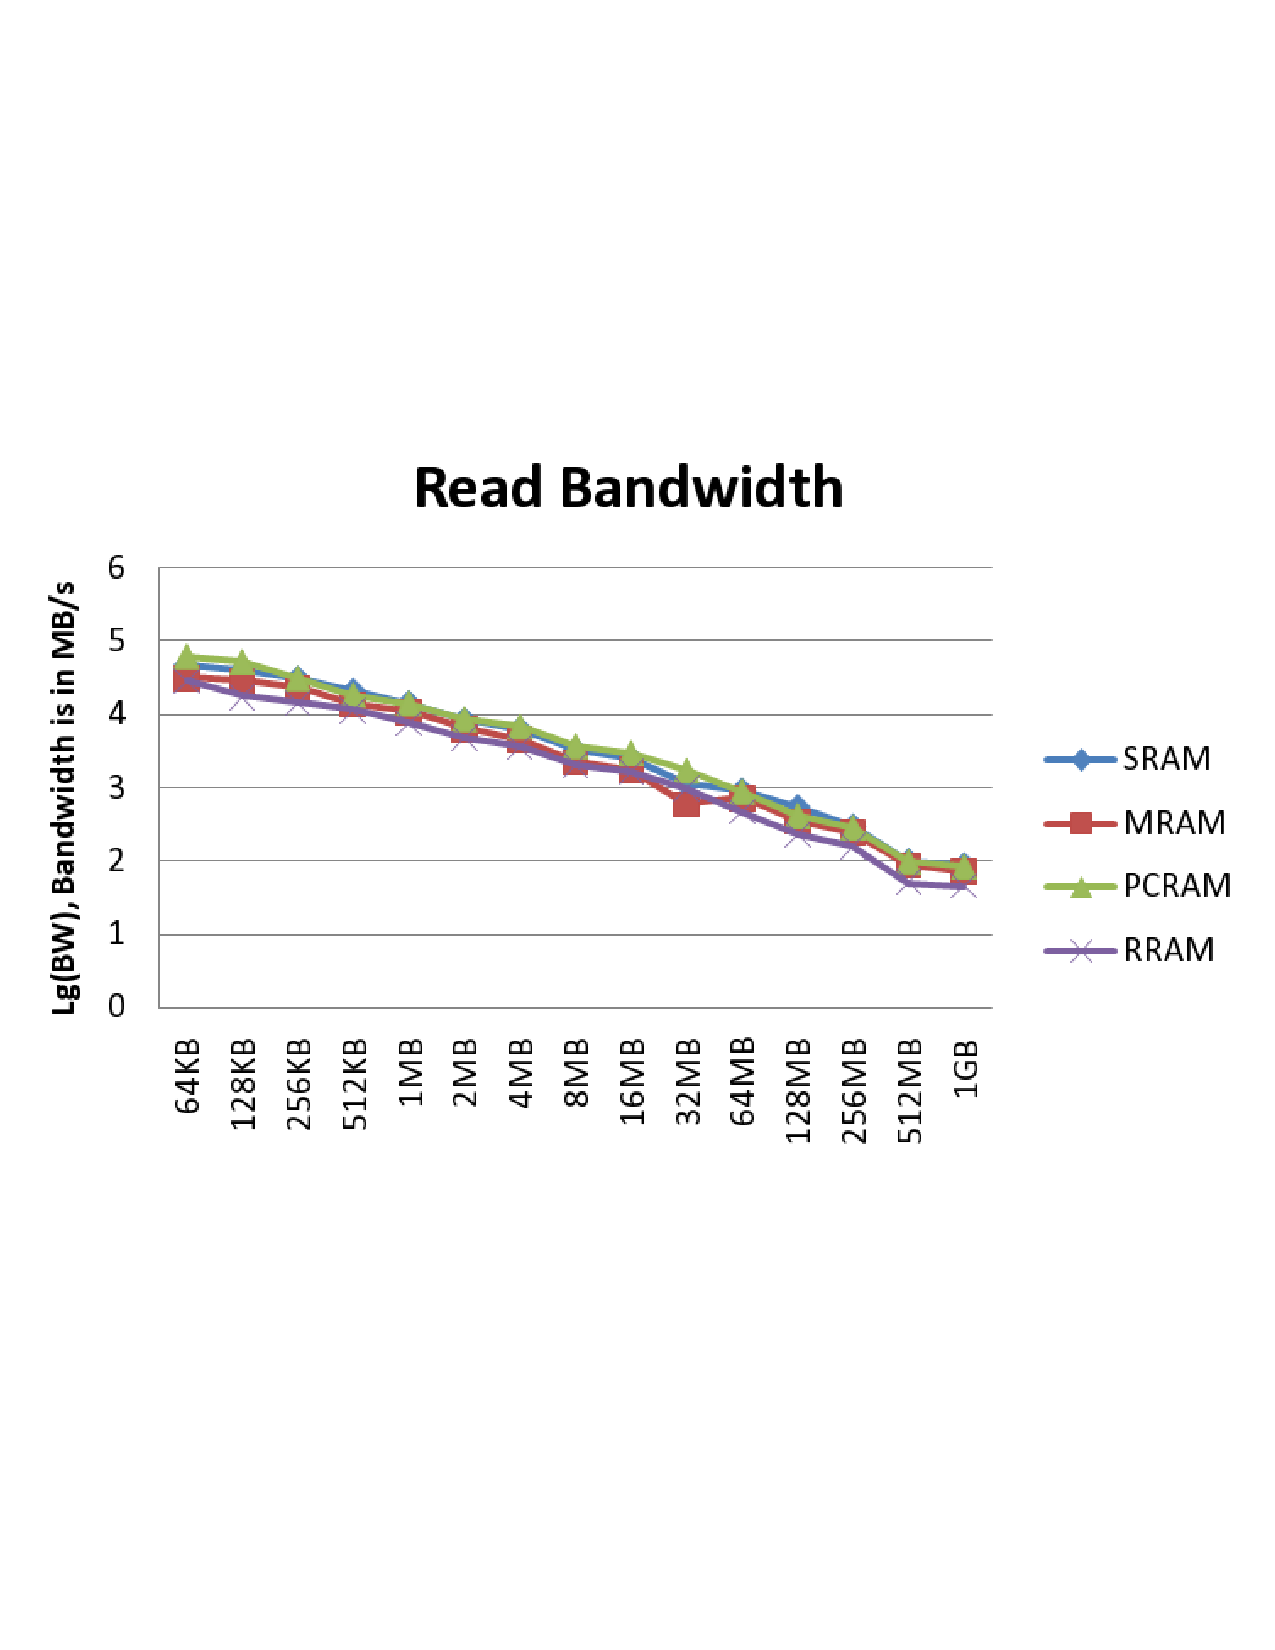
\includegraphics[width=3in]{figures/read-bw}
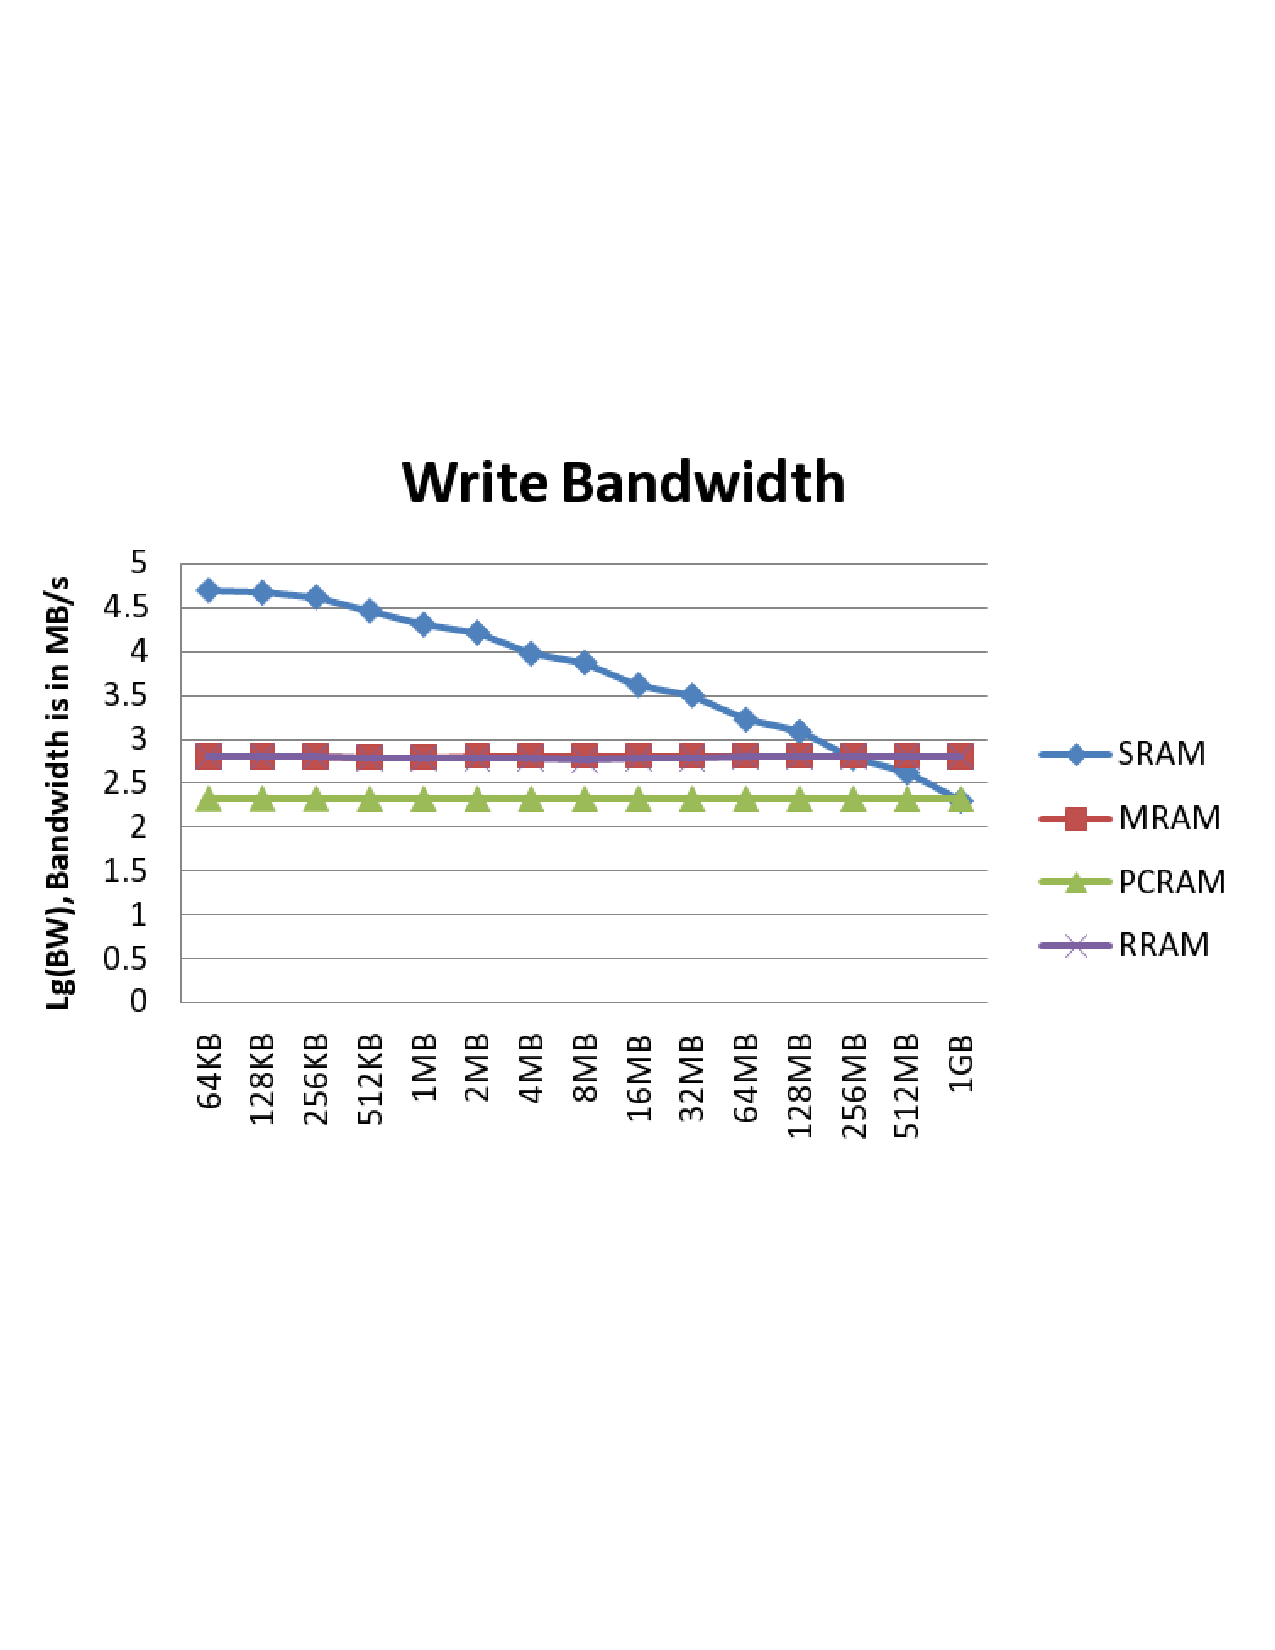
\includegraphics[width=3in]{figures/write-bw}\\

\vspace*{-1in}
\hspace{0.02in}
\makebox[3in][l]{\textcolor [rgb]{0,0,0} {\bf (a)}}
\makebox[3in][l]{\textcolor [rgb]{0,0,0} {\bf (b)}}

\caption{Read and write bandwidths provided by different memory technologies.
(a) Read bandwidth provided by different memory technologes. (b) Write bandwidth
provided by different memory technologies.}
\label{fig:memory-bw}
\end{figure*}

\begin{figure*}[htbp]
% The "!" means to maintain the aspect ratio.   
\centering
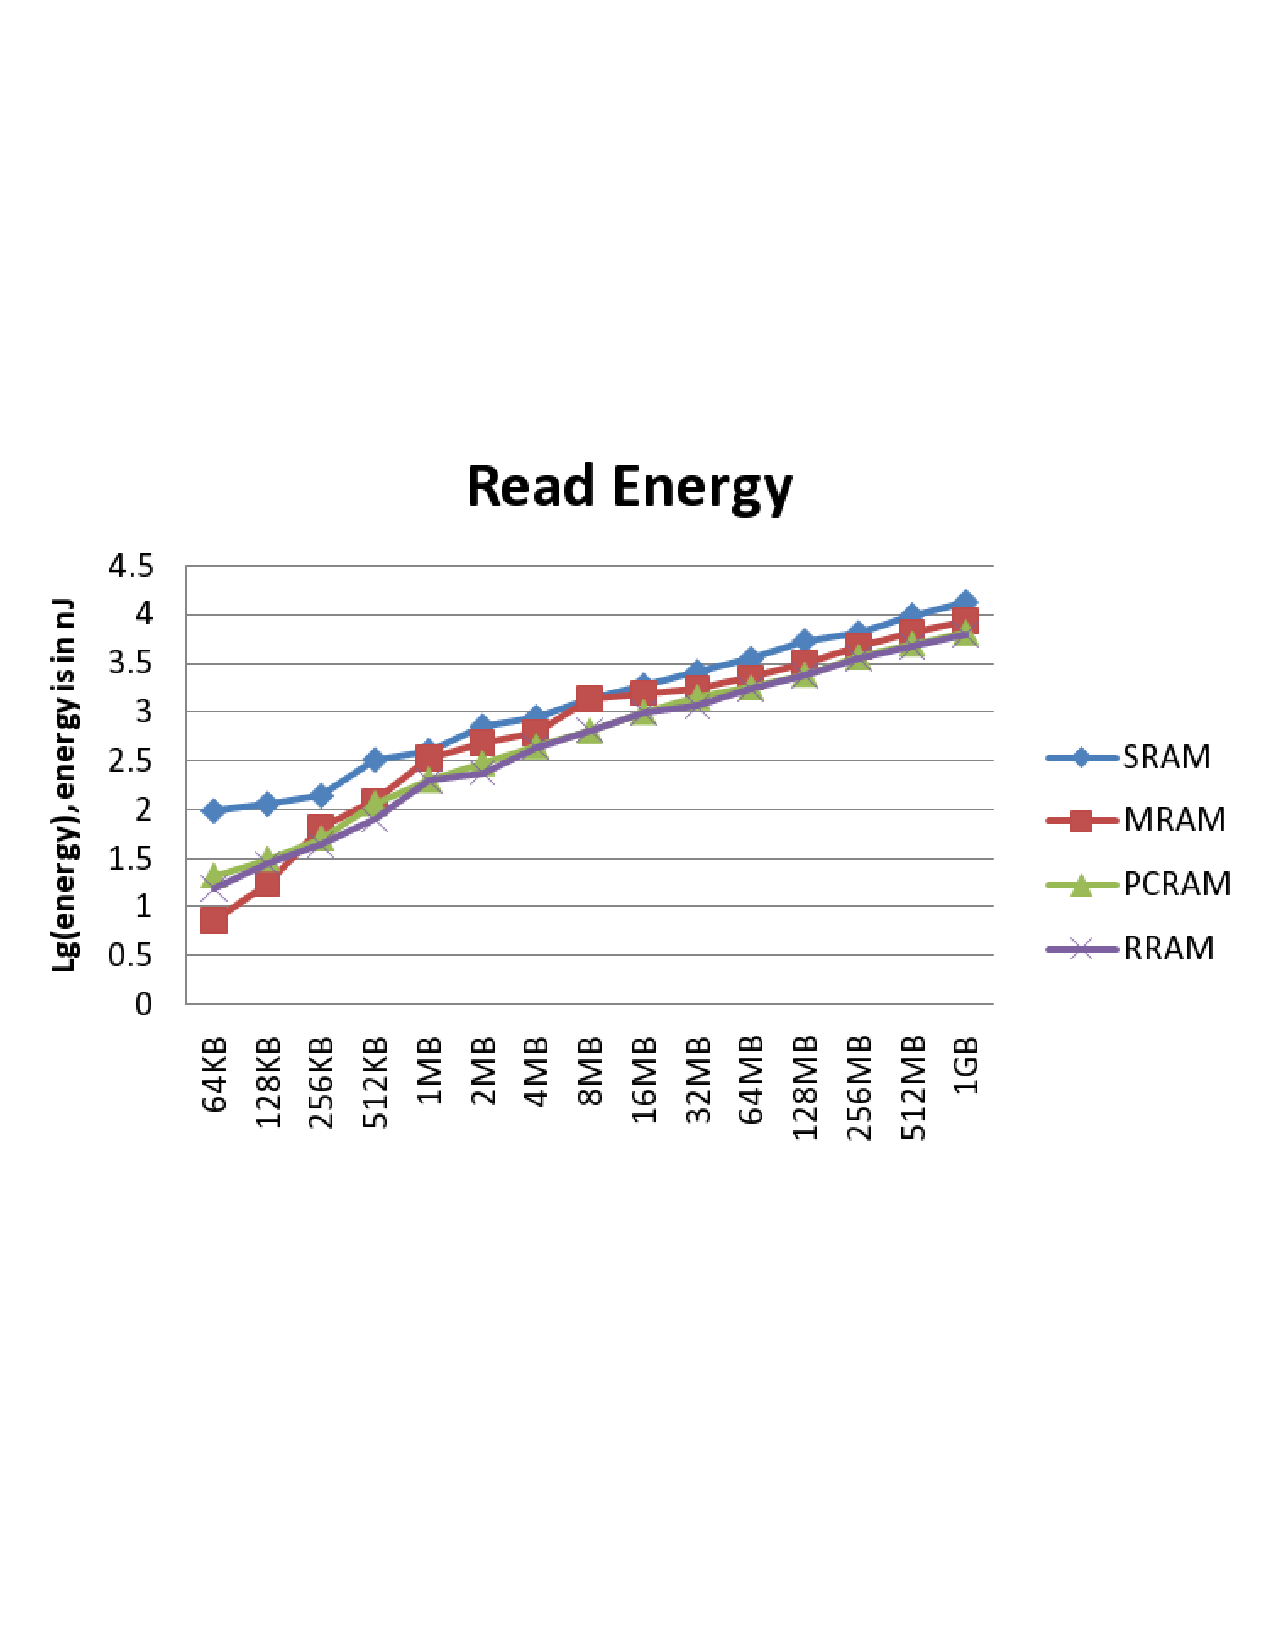
\includegraphics[width=2in]{figures/read-energy}
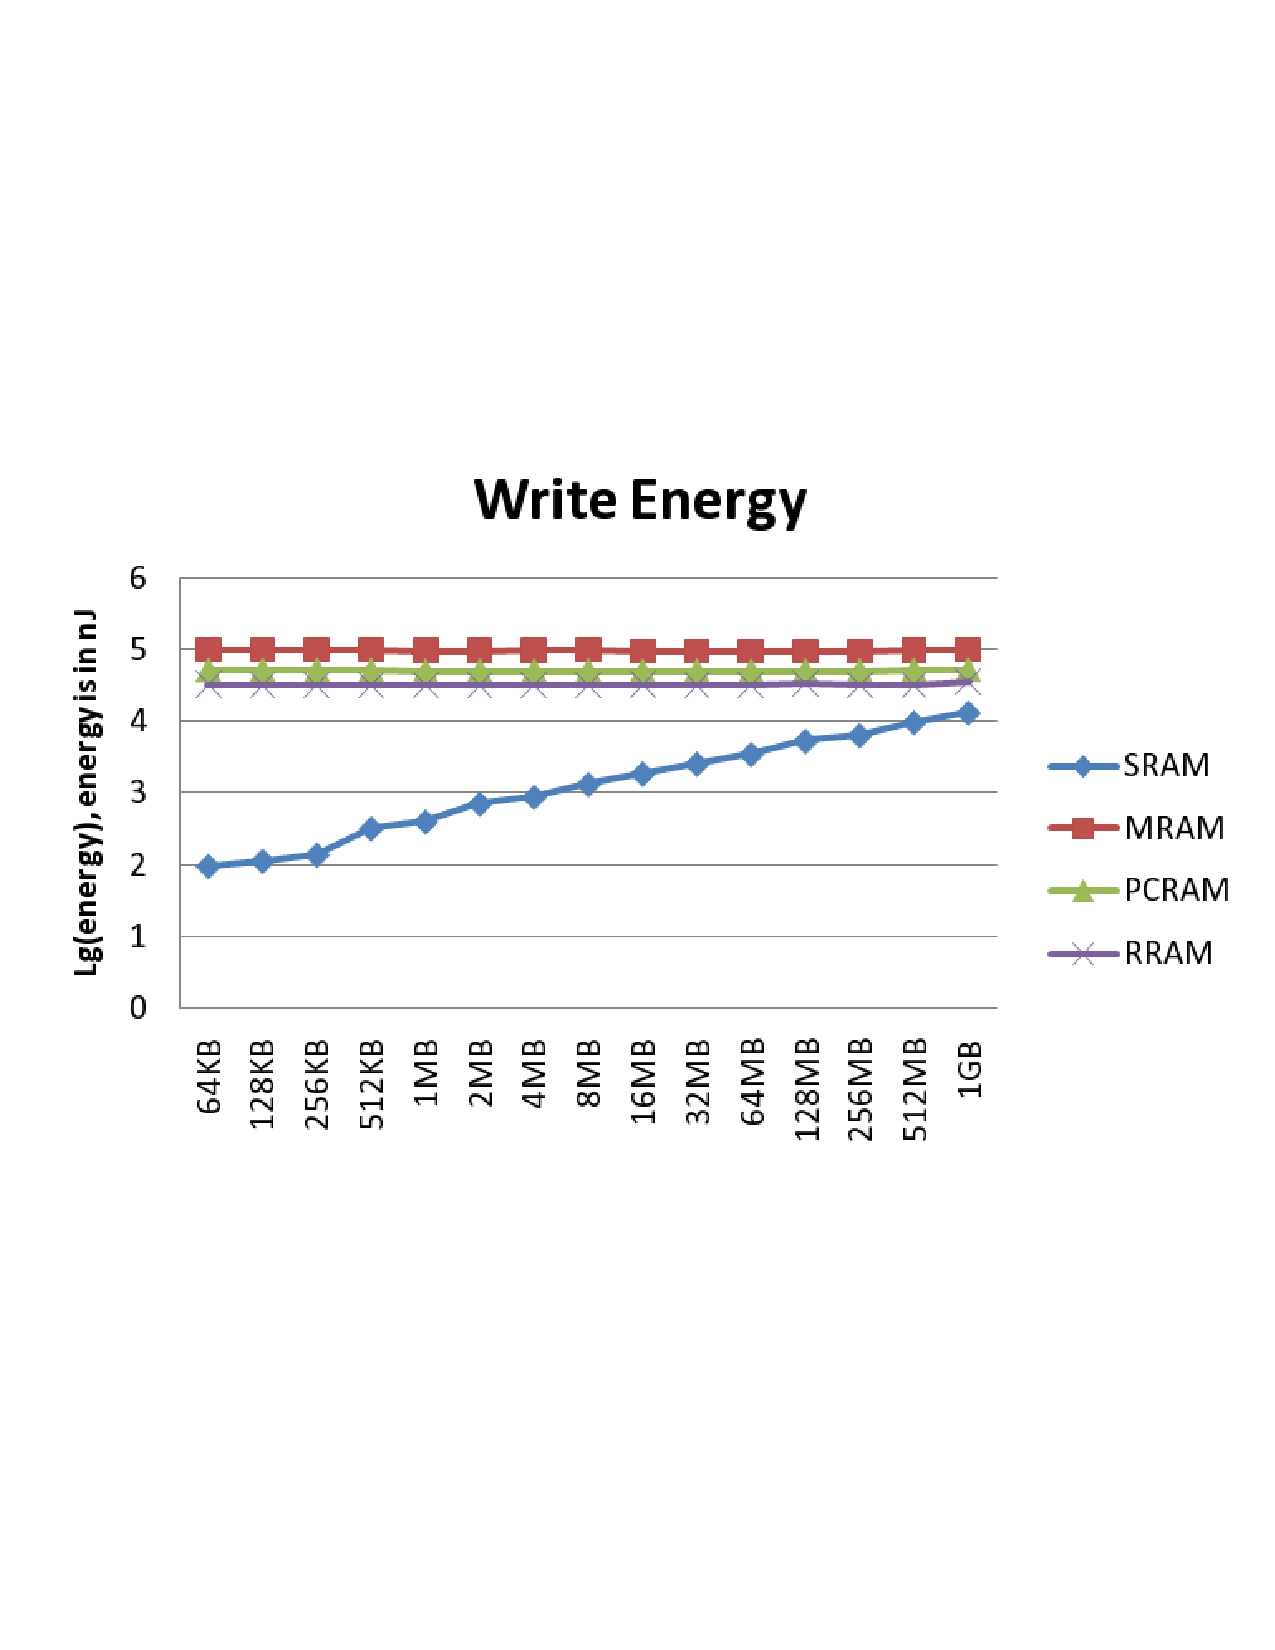
\includegraphics[width=2in]{figures/write-energy}
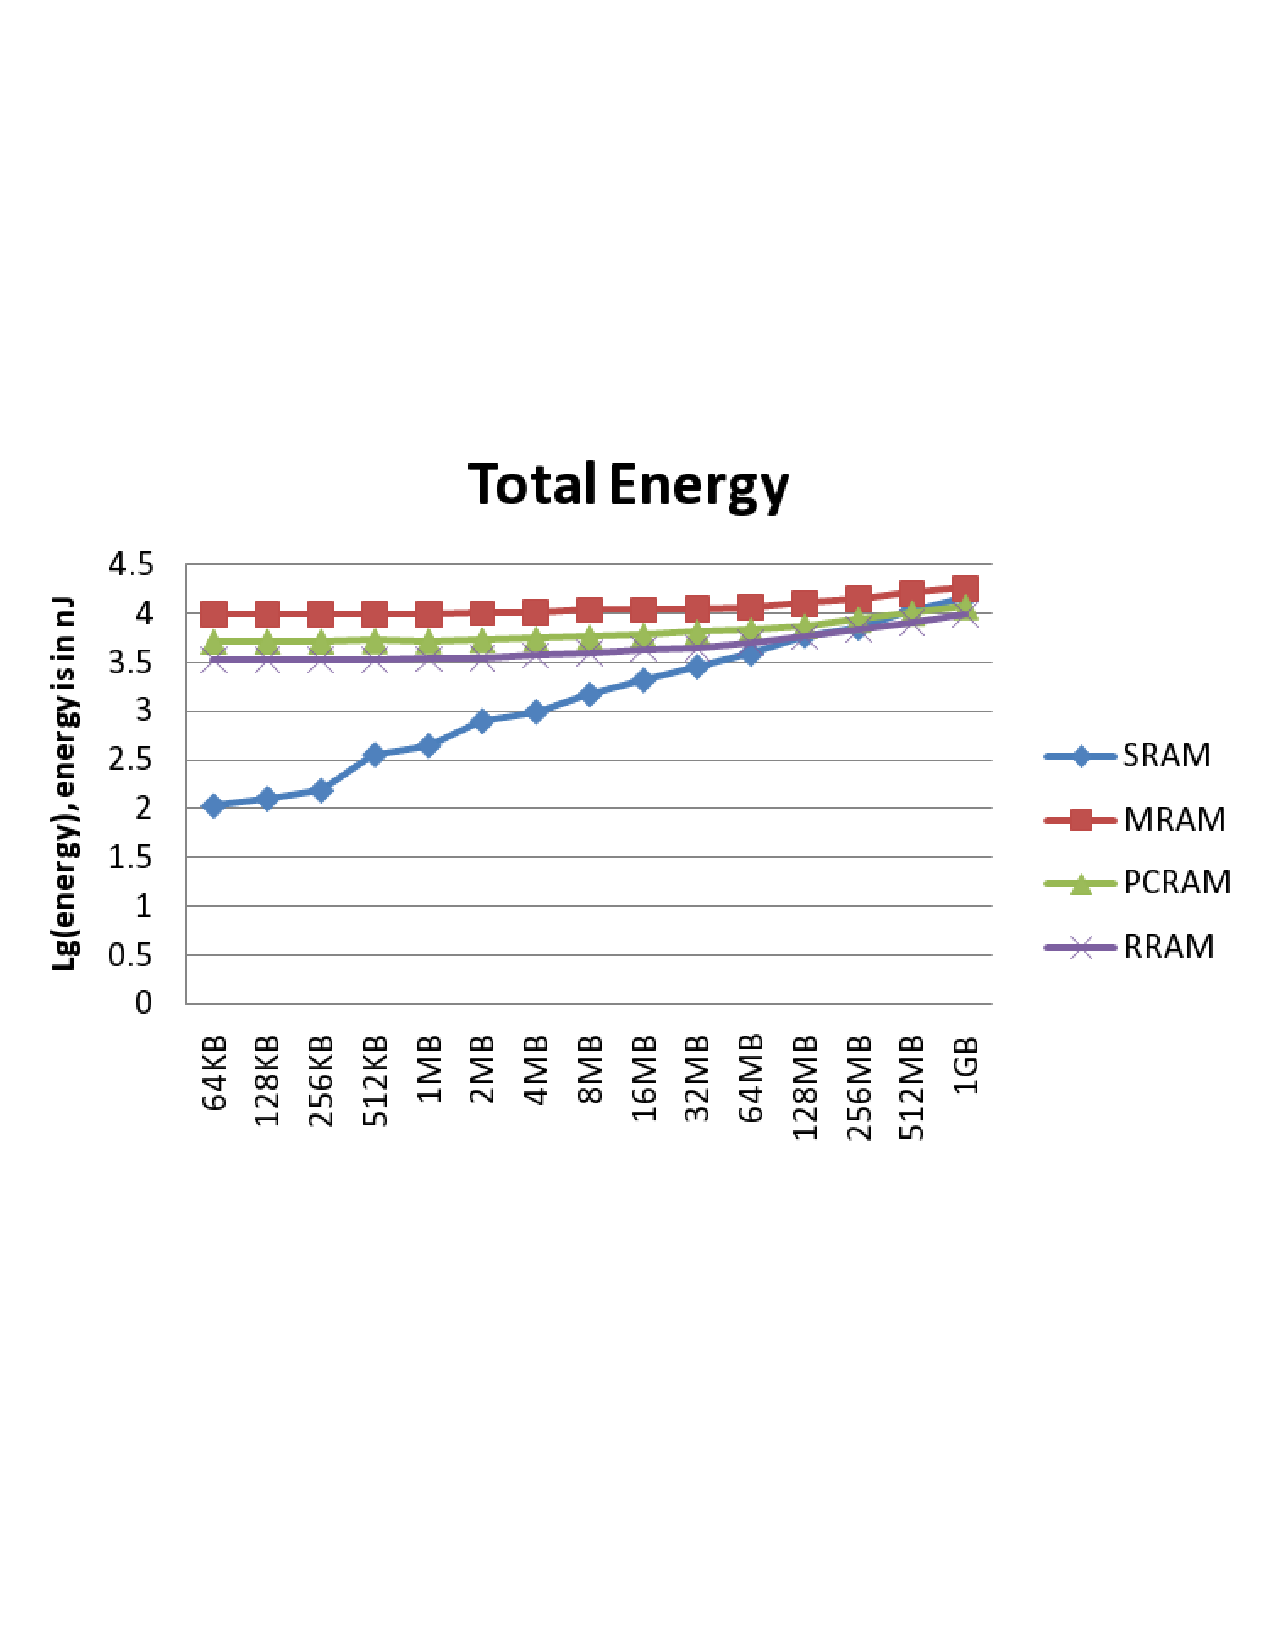
\includegraphics[width=2in]{figures/total-energy}\\

\vspace*{-0.5in}
\hspace{0.02in}
\makebox[2in][l]{\textcolor [rgb]{0,0,0} {\bf (a)}}
\makebox[2in][l]{\textcolor [rgb]{0,0,0} {\bf (b)}}
\makebox[2in][l]{\textcolor [rgb]{0,0,0} {\bf (c)}}

\caption{Dynamic energy consumption with the provided bandwidths of different
  memory technologies. (a) Read energy of different memory technologes. (b)
  Write energy of different memory technologies. (c) Total energy consumption
  (with 10\% write) of different memory technologies.}
\label{fig:memory-energy}
\end{figure*}

First of all, we estimate the read and write bandwidths that can be provided by
different memory technologies. Figure~\ref{fig:memory-bw} shows the results,
with both x- and y-values in \emph{log} scale. The figure illustrates both the
provided read and write bandwidth as a function of memory capacity. Each of the
memory technologies actually provide nearly the same read bandwidths, as is
shown in figure~\ref{fig:memory-bw}(a). On the other hand, a straight forward
observation from figure~\ref{fig:memory-bw}(b) is that the write bandwidth
varies among different memory technologies. The shape of the SRAM write
bandwidth curve is very similar to the read bandwidth curve. The write bandwidth
curves of the other three memory technologies appear to be very different. The
reason is that write latencies of the three non-volatile memories are much
higher than read latencies. Another observation from
figure~\ref{fig:memory-bw}(b) is that the curves cross to each other at
different locations. Based on these two observations, we would like to design a
bandwidth-aware hybrid memory hierarchy, which always provides the high memory
bandwidth with the given capacity. For example, we probably would like to use
1) SRAM when the memory capacity is under 256MB, 2) MRAM or RRAM between
256MB and 1GB (if only bandwidth is considered), and 3) PCRAM when the memory
cacity is over 1GB. 

In addition, we would like to put an upper bound to the total dynamic energy
consumption of the memory hierarchy. Figure~\ref{fig:memory-energy} shows the
estimation of dynamic power consumptions of different memory technologies with
the provided bandwidths. In figure~\ref{fig:memory-energy}(c), we estimate the total
dynamic energy with 10\% write activities.

% \bibliographystyle{IEEEtran}
\bibliographystyle{latex8}
\bibliography{./bib/ref}

\end{large}

\end{document}